\let\negmedspace\undefined
\let\negthickspace\undefined
\documentclass[journal]{IEEEtran}
\usepackage[a5paper, margin=10mm, onecolumn]{geometry}
\usepackage{lmodern} % Ensure lmodern is loaded for pdflatex
\usepackage{tfrupee} % Include tfrupee package

\setlength{\headheight}{1cm} % Set the height of the header box
\setlength{\headsep}{0mm}     % Set the distance between the header box and the top of the text

\usepackage{gvv-book}
\usepackage{gvv}
\usepackage{cite}
\usepackage{amsmath,amssymb,amsfonts,amsthm}
\usepackage{algorithmic}
\usepackage{graphicx}
\usepackage{textcomp}
\usepackage{xcolor}
\usepackage{txfonts}
\usepackage{listings}
\usepackage{enumitem}
\usepackage{mathtools}
\usepackage{gensymb}
\usepackage{comment}
\usepackage[breaklinks=true]{hyperref}
\usepackage{tkz-euclide} 
\usepackage{listings}
\def\inputGnumericTable{}                                 
\usepackage[latin1]{inputenc}                                
\usepackage{color}                                            
\usepackage{array}                                            
\usepackage{longtable}                                       
\usepackage{calc}                                             
\usepackage{multirow}                                         
\usepackage{hhline}                                           
\usepackage{ifthen}                                           
\usepackage{lscape}

\begin{document}

\bibliographystyle{IEEEtran}
\vspace{3cm}

\title{10.4.ex.11}
\author{EE24BTECH11014 - Deepak Ahirwar }
% \maketitle
% \newpage
% \bigskip
{\let\newpage\relax\maketitle}

\renewcommand{\thefigure}{\theenumi}
\renewcommand{\thetable}{\theenumi}
\setlength{\intextsep}{10pt} % Space between text and floats

\renewcommand{\thefigure}{\theenumi}
\renewcommand{\thetable}{\theenumi}
\setlength{\intextsep}{10pt} % Space between text and floats

\textbf{Question}: Find two consecutive odd positive integers, sum of whose squares is $290$.\\

\textbf{Solution}:
Let the smaller of the two consecutive odd positive integers be \( x \). Then, the second integer will be \( x + 2 \). 
\\According to the question:
\begin{align}
x^2 + (x + 2)^2 &= 290 \label{eq1}
\end{align}

Simplify:
\begin{align}
x^2 + x^2 + 4x + 4 &= 290 \label{eq2} \\
2x^2 + 4x + 4 - 290 &= 0 \label{eq3} \\
2x^2 + 4x - 286 &= 0 \label{eq4}
\end{align}

Divide the equation by 2:
\begin{align}
x^2 + 2x - 143 &= 0 \label{eq5}
\end{align}

Using the quadratic formula:
\begin{align}
x &= \frac{-b \pm \sqrt{b^2 - 4ac}}{2a} \label{eq6}
\end{align}
Here, \( a = 1 \), \( b = 2 \), and \( c = -143 \):
\begin{align}
x &= \frac{-2 \pm \sqrt{2^2 - 4(1)(-143)}}{2(1)} \label{eq7} \\
x &= \frac{-2 \pm \sqrt{4 + 572}}{2} \label{eq8} \\
x &= \frac{-2 \pm \sqrt{576}}{2} \label{eq9} \\
x &= \frac{-2 + 24}{2} \quad \text{or} \quad x = \frac{-2 - 24}{2} \label{eq10} \\
x &= 11 \quad \text{or} \quad x = -13 \label{eq11}
\end{align}

Since \( x \) is given to be an odd positive integer:
\begin{align}
x &= 11 \label{eq12}
\end{align}

Thus, the two consecutive odd integers are \( 11 \) and \( 13 \).\\



\textbf{CODING LOGIC:-}


\textbf{Eigen value method}
\begin{enumerate}
\item Characteristics polynomial is given by
\begin{align}
 p(x)=a_nx^n+a_{n-1}x^{n-1}+\cdots +a_1x+a_0   
\end{align}
where $a_n \neq 0$
\item Divide Characteristics equation by $a_n$
\begin{align}
    p(x)= a_nx^n+a_{n-1}x^{n-1}+\cdots +a_1x+a_0     \\
    p(x)=x^n+\frac{a_{n-1}}{a_n}x^{n-1}+\cdots +\frac{a_1}{a_n}x+\frac{a_0}{a_n}
\end{align}
\item Companion Matrix of characteristic polynomial is given by:\\
Let
\begin{align}
    \begin{bmatrix}
0 & 1 & 0 & \cdots & 0 \\
0 & 0 & 1 & \cdots & 0 \\
\vdots & \vdots & \vdots & \ddots & \vdots \\
0 & 0 & 0 & \cdots & 1 \\
-\frac{a_0}{a_n} & -\frac{a_1}{a_n} & -\frac{a_2}{a_n} & \cdots & -\frac{a_{n-1}}{a_n}
\end{bmatrix}
\end{align}
\item QR decomposition 
\begin{align}
A = QR
\end{align}
\begin{enumerate}
    \item $Q$ is an $ m \times n $ orthogonal matrix
    \item $R$ is an $n \times n$ upper triangular matrix.
\end{enumerate}
Given a matrix $ A = [a_1, a_2, \dots, an] $, where each $ a_i $ is a column vector of size $ m \times 1 $.

\item Normalize the first column of $A$:
\begin{align}
q_1 = \frac{a_1}{\norm{a_1}}
\end{align}

\item  For each subsequent column $ a_i $, subtract the projections of the previously obtained orthonormal vectors from $ a_i $ :
\begin{align}
a_i' = a_i - \sum_{k=1}^{i-1} \langle a_i, q_k \rangle q_k
\end{align}
Normalize the result to obtain the next column of \( Q \):
\begin{align}
q_i = \frac{a_i'}{\norm{a_i'}}
\end{align}

Repeat this process for all columns of \( A \).
\item Finding $R$:- \\
After constructing the ortho-normal columns $ q_1, q_2, \dots, q_n $ of $Q$, we can compute the elements of $R$ by taking the dot product of the original columns of $A$ with the columns of $Q$:

\begin{align}
    r_{ij} = \langle a_j, q_i \rangle \text{ , for  }  i \leq j 
\end{align}
\item \textbf{QR-Algorithm}\\
\begin{enumerate}
\item Initialization \\
Let $A_0 = A $, where $A$ is the given matrix.

\item QR Decomposition \\
For each iteration $ k = 0, 1, 2, \dots $:
\begin{enumerate}
    \item Compute the QR decomposition of \( A_k \), such that:
    \begin{align}
    A_k = Q_k R_k
    \end{align}
    where:
    \begin{enumerate}
        \item $Q_k $ is an orthogonal matrix ($ Q_k^\top Q_k = I $).
        \item $ R_k $ is an upper triangular matrix.
    \end{enumerate}
    The decomposition ensures $ A_k = Q_k R_k $.

    \item Form the next matrix \( A_{k+1} \) as:
    \begin{align}
    A_{k+1} = R_k Q_k
    \end{align}
\end{enumerate}
\item Convergence\\
Repeat Step 2 until $ A_k $ converges to an upper triangular matrix $ T $. The diagonal entries of $T$ are the eigenvalues of $A$.\\
\item The eigenvalues of matrix will be the roots of the equation.

\end{enumerate}



\end{enumerate}

\begin{figure}[h!]
   \centering
   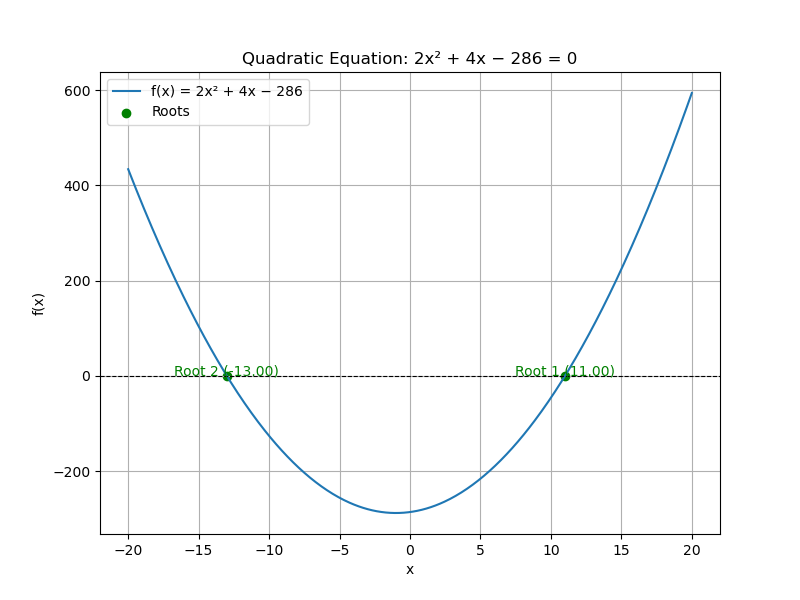
\includegraphics[width=0.7\linewidth]{figs/Figure_1.png}
\end{figure}
		
		

\end{document}_
